\newpage
\section{User}

\subsection{How does it works?}

In the Salespointframework there is one \code{PersistenceUsermanger}, but it is not a singelton. You can instanciet a new
\code{PersistenceUsermanger} whenever you need it (it allways manages the same data!).
The Usermanger ist the main part of the UserPackage. It connects all parts:
You can adds and removes User to/from the System and also adds and removes \code{UserCapabilities} of the Users in the System

\begin{figure}[ht]
	\centering
  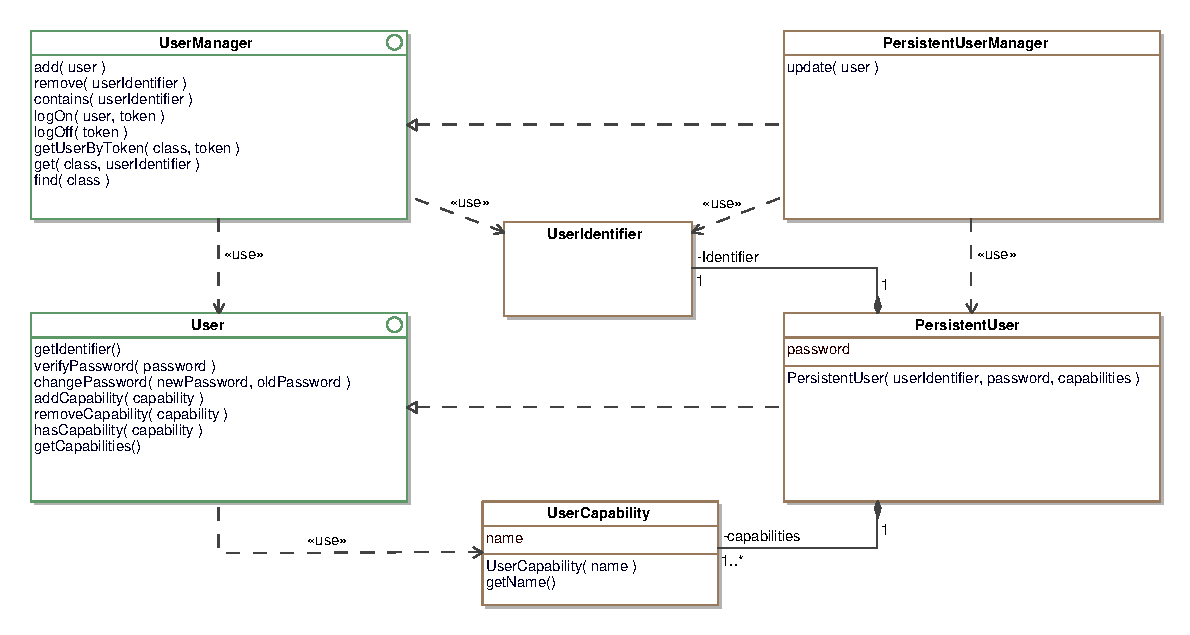
\includegraphics[width=1.0\textwidth]{images/User_Overview.eps}
	\label{user_overview}
	\caption{User - Class Overview}
\end{figure}

\subsection{Ensure correct Data}
To ensure you have the correct data in your system you should only access \code{users} and their \code{UserCapabilities} via the \code{PersistenceUsermanger}:

During the process of adding a user to the system the \code{PersistenceUsermanger} garanties that there will be no duplicate Users. If you try to add a \code{User} with an \code{UserIdentifier} that is already in the system a DuplicateUserException will be thrown. This will help you to identifie \code{Users} correctly, e.g. during the login process.

You should notice that it is not possible to remove Users with open \code{orders}! You have to close/finish them before.

You only able to add a \code{UserCapability} to an \code{user}, which is in they system. Otherwise you will get an UnknownUserException.
This ensures that a new \code{user} will have no \code{UserCapabilities}.

\subsection{Why are there so many users?}
First of all we do have the \code{User} class. This is the user interface with all basic methodes. The are implemented in the
\code{PersistenceUser} and also the basic attributes of an user.
The subclasses of the \code{PersistenceUser} are the \code{AbstractEmployee} and the \code{AbstractCustomer}.
\code{AbstractEmployee}: A spezial User who also has an salary. This helps to work together with the \code{Accountency}.
\code{AbstractEmployee}: This Class is not very usefule, also is shows the user of the Framework that there could be different subclasses of the \code{PersistenceUser}.


\subsection{login}

ASK PAUL!





